\documentclass[11pt,a4paper]{article}

\usepackage{graphicx}
\usepackage{mathtools,amssymb}

\usepackage{amsthm}
\theoremstyle{definition}
\newtheorem{definition}{Definition}[section]

\usepackage{enumitem}
\usepackage{float}
\usepackage[number-unit-product = {\ }]{siunitx}
\usepackage{setspace}
\usepackage{caption}
\captionsetup{skip = 10 pt, font=small}

\usepackage[CJKmath=true,AutoFakeBold=3,AutoFakeSlant=.2]{xeCJK}
\setCJKmainfont{標楷體}
\setCJKsansfont{微軟正黑體} 
\setCJKmonofont{標楷體}
\newCJKfontfamily\Kai{標楷體}
\newCJKfontfamily\Hei{微軟正黑體}
\newCJKfontfamily\NewMing{新細明體} 
\XeTeXlinebreaklocale "zh"

\usepackage[backend=biber, style=numeric, sorting=none]{biblatex}
\addbibresource{references.bib} % 告訴 LaTeX 參考資料檔案的位置

\usepackage[colorlinks=true,
    linkcolor=blue,    % 目錄和章節標題連結 = 黑色
    citecolor=blue,     % 文獻引用超連結 = 藍色
    urlcolor=blue,      % 網址超連結 = 藍色
    filecolor=blue,     % 檔案超連結 = 藍色
    anchorcolor=blue    % 其他定位點 = 藍色
]{hyperref}

\begin{document}

    \section{實驗數據與分析}

        \subsection{實驗A:向心力和角速度的關係}

        此實驗固定滑塊質量$m$及繩長$r$,角速度向心力$F$與角速度$\omega$的關係
        \par
        在進行實驗時,我們將電源供應器的最大電壓固定設為
        \SI{10}{\volt},透過改變電流 $I$ 來改變旋轉角速度$\omega$,如此一來便可在控制角速度的同時避免超過馬達所能承受的電壓上限。

        \begin{gather}
            F = mr\omega^2 - f
        \end{gather}

        其中$F$為繩張力,$f$為摩擦力,經由摩擦力公式

        \begin{gather}
            f \leq m g \mu
        \end{gather}

        其中 $g$ 為重力場強度,此處採用標準重力加速度近似值 $g = \SI{9.7890191}{\meter\per\second\squared}$\cite{TWD2000},$\mu$ 為鐵架和旋轉滑塊的靜摩擦係數,若假設平衡時的摩擦力為最大靜摩擦力,則

        \begin{gather}
            F = mr\omega^2 - m g \mu
        \end{gather}

        \begin{figure}[H]
            \centering
            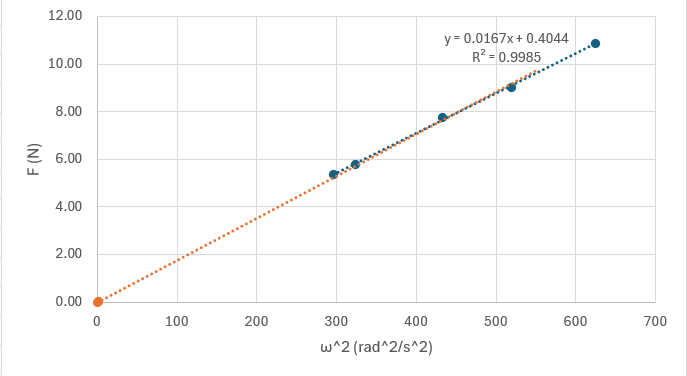
\includegraphics[width=0.8\textwidth]{實驗A數據.png}
            \caption{實驗A數據以力$F$對旋轉半徑$r$作圖。我們固定滑塊質量為$m = 97.74\ g$,旋轉半徑 $r = 18.10\ cm$。,得到斜率為\SI{0.0167}{\newton\second\squared},截距為\SI{0.40}{\newton}。}
            \label{fig:實驗A數據 Excel原始數據}
        \end{figure}
    
        由先前推導的 $F = mr\omega^2 - m g \mu$ 可以知道 \autoref{fig:實驗A數據 Excel原始數據} 的斜率理論值推出在圖表一當中的的理論斜率
        \begin{equation}
            mr = (97.74 \times 10^{-3}\ \si{\kilogram}) \times (18.10 \times 10^{-2}\ \si{\meter}) = 0.01769\ \si{\kilogram\meter}
        \end{equation}

        其中實驗斜率為 $0.0167$。與理論誤差為

        \begin{equation} 
            \frac{0.01769 - 0.0167}{0.01769} \times 100\% = 5.6\% 
        \end{equation}

        理論上,應為本實驗的截距應為 $-mg\mu$ ,然而\autoref{fig:實驗A數據 Excel原始數據} 的截距卻為正值,因此無法計算出其靜摩擦係數。
    
        \subsection{實驗B:向心力和半徑的關係}
            此實驗是要改變旋轉半徑$r$, 觀察其與向心力$F$的關係。滑塊質量$m$,角速度$\omega$為控制變因因此固定固定。在實驗過程中發現,改變繩長時若不調整電流,角速度$\omega$也會跟著改變,因此我們在每次改變繩長的時候都會重新微調電源供應器的電流以維持角速度$\omega$。

            \begin{figure}[H]
                \centering
                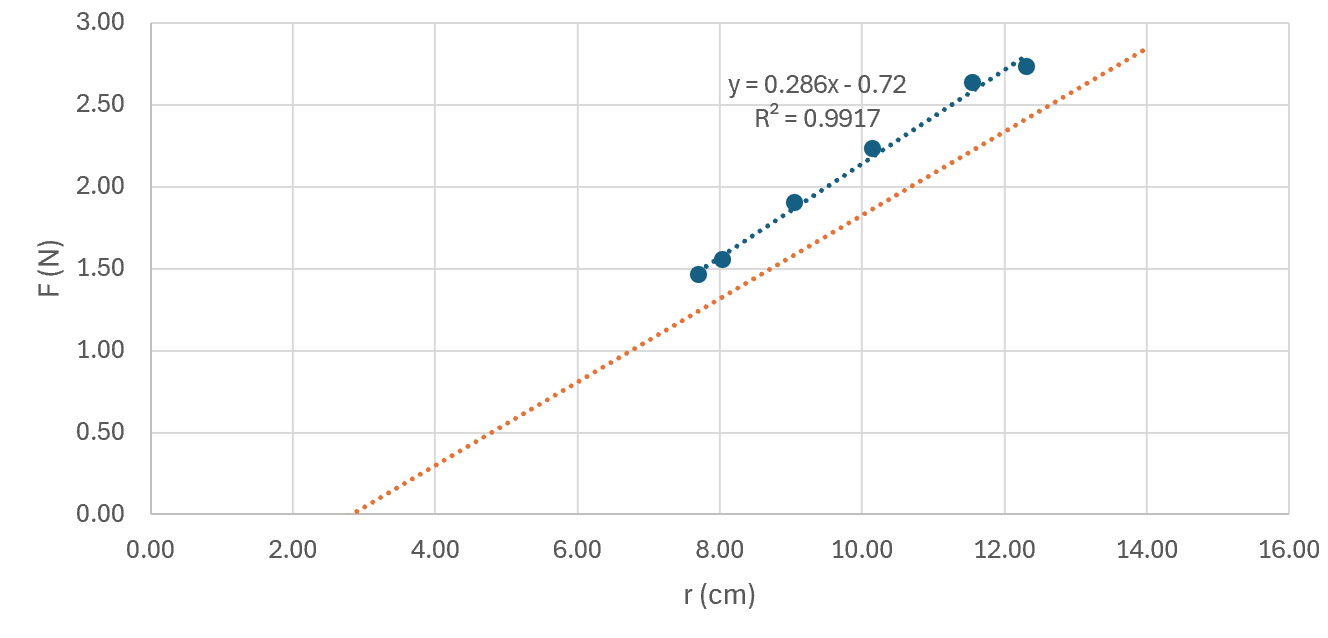
\includegraphics[width=0.8\textwidth]{實驗B數據.png}
                \caption{實驗B數據以力$F$對旋轉半徑$r$作圖。我們固定角速度$\omega = \SI{18.0}{\radian\per\second}$,滑塊質量$m = \SI{78.47}{\gram}$,得到斜率為\SI{0.286}{\newton\per\centi\meter},截距為\SI{0.72}{\newton}。}
                \label{fig:實驗B數據 Excel原始數據}
            \end{figure}

            由先前推導的 $F = mr\omega^2 - m g \mu$ 可以知道 \autoref{fig:實驗B數據 Excel原始數據} 的斜率理論值
            \begin{equation}
                m\omega^2 = (78.47 \times 10^{-3}\ \si{\kilogram}) \times (18.0\ \si{\radian\per\second})^2 = 25.4\ \si{\newton\per\meter}
            \end{equation}

            其中實驗所得斜率為 $\SI{28.6}{\newton\per\meter}$。對理論值的誤差為

            \begin{equation} 
                \frac{\SI{28.6}{\newton\per\meter} - \SI{25.4}{\newton\per\meter}}{\SI{25.4}{\newton\per\meter}} \times 100\% = 13\% 
            \end{equation}

            另外我們以截距計算鐵架與滑塊的靜摩擦係數。

            \begin{gather}
                -mg\mu = \SI{-0.72}{\newton}\\
                \Rightarrow \mu = \frac{\SI{0.72}{\newton}}{mg} = \frac{0.72\ \si{\newton}}{(78.47 \times 10^{-3}\ \si{\kilogram}) \times 9.789 019 1\ \si{\meter\per\second\squared}} = 0.94
            \end{gather}

        \subsection{實驗C:向心力與質量的關係}

            本實驗固定旋轉半徑$r$及角速度$\omega$觀察其與向心力$F$對滑塊質量$m$的關係。與實驗B相同,我們每次測量皆有校正電流,以確保每次的角速度一樣。

            \begin{figure}[H]
                \centering
                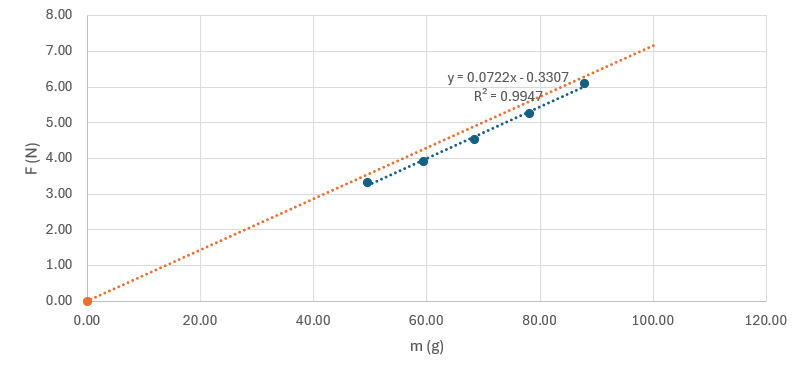
\includegraphics[width=0.8\textwidth]{實驗C數據.png}
                \caption{實驗C數據以力$F$對滑塊質量$m$作圖。我們固定角速度 $\omega = \SI{20.0}{\radian\per\second}$ ,旋轉半徑$r = \SI{17.90}{\centi\meter}$,得到斜率為\SI{0.07220}{\newton\per\gram},截距為\SI{0.33}{\newton}。}
                \label{fig:實驗C數據 Excel原始數據}
            \end{figure}
                        
            由先前推導的 $F = m (r\omega^2 - g \mu)$ 可以知道 \autoref{fig:實驗C數據 Excel原始數據} 的斜率為 $r\omega^2 - g \mu$,然而因為實驗A、B對摩擦力的推測相當不一致,故忽略摩擦力,取斜率的理論值

            \begin{equation}
                r\omega^2 = (17.90 \times 10^{-2}\ \si{\meter}) \times (20.0\ \si{\radian\per\second})^2 = 71.6\ \si{\newton\per\kilogram}
            \end{equation}

            其中實驗所得斜率為 $\SI{72.20}{\newton\per\kilogram}$。對理論值的誤差為
            
            \begin{equation} 
                \frac{\SI{72.20}{\newton\per\kilogram} - \SI{71.6}{\newton\per\kilogram}}{\SI{71.6}{\newton\per\kilogram}} \times 100\% = 0.8\% 
            \end{equation}

        \subsection{實驗A、實驗B、實驗C斜率之討論}

            在三個實驗中, 實驗A的\autoref{fig:實驗A數據 Excel原始數據} 、 實驗B的\autoref{fig:實驗B數據 Excel原始數據} 中的斜率對理論值誤差分別為 5.6\% 和 13\%,皆有明顯正偏差,而實驗C的 \autoref{fig:實驗C數據 Excel原始數據} 斜率對理論值雖為 +0.8\% ,然而考慮我們將斜率理論值由 $r\omega^2 - g \mu$ 省略了 $-g \mu$ 改為僅計算 $r\omega^2$ 為理論值,亦代表其斜率有正偏差。由於三組實驗 \autoref{fig:實驗A數據 Excel原始數據} 、 \autoref{fig:實驗B數據 Excel原始數據} 、 \autoref{fig:實驗C數據 Excel原始數據} 的縱軸皆為繩張力,這代表力隨角速度、旋轉半徑、的滑塊質量增大的上升幅度都較大,我們推測原因為線並未拉直如\autoref{fig:纜線傾斜示意圖} 所示。

            \begin{figure}[H]
                \centering
                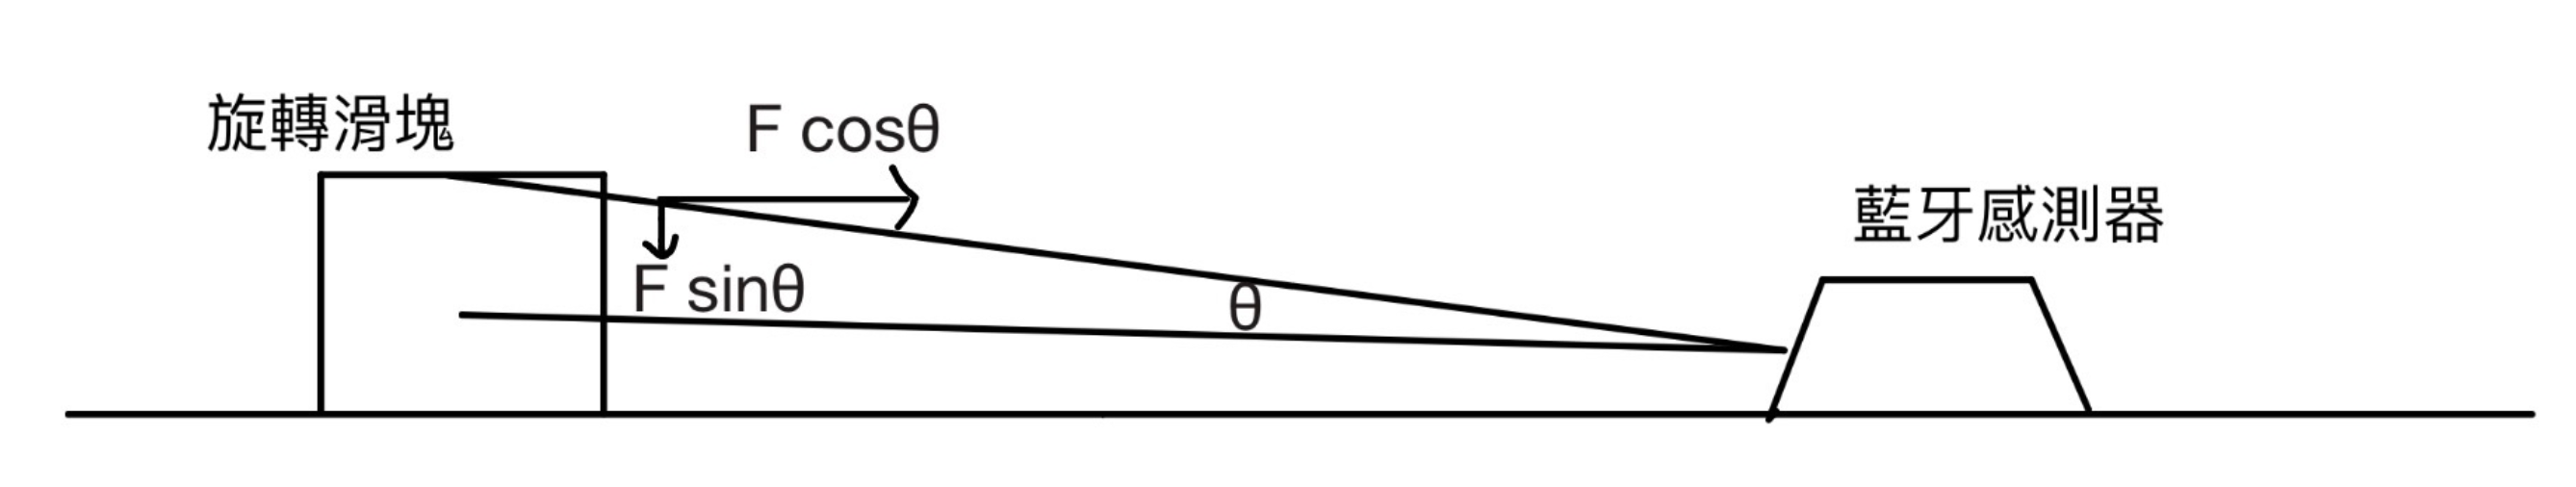
\includegraphics[width=0.8\textwidth]{纜線傾斜示意圖.png}
                \caption{纜線傾斜示意圖。此圖顯示一個在垂直方向傾斜的纜線,其中 $F$ 為纜線繩張力,實際為只有 $F \cos{\theta} $為向心力貢獻。本圖僅畫出垂直方向的傾斜的影響,而實驗時水平方向也可能傾斜,其影響相同。}
                \label{fig:纜線傾斜示意圖}
            \end{figure}

            若考慮纜繩的傾斜,則原本 $F = mr\omega^2 - m g \mu$ 應改為 
            
            \begin{gather}
                F \cos{\theta} = mr\omega^2 - m g \mu\\
                \Rightarrow F = \frac{mr\omega^2}{\cos{\theta}} - \frac{mg\mu}{\cos{\theta}}
            \end{gather}

            然而根據此方式計算出的 $\theta$ 在實驗A為

            \begin{equation}
               \theta = \arccos\left( \frac{1}{1 + 0.056} \right) = \ang{18.74}
            \end{equation}

            而在實驗B則為

            \begin{equation}
               \theta = \arccos\left( \frac{1}{1 + 0.13} \right) = \ang{27.8}
            \end{equation}

            雖然此模型可以解釋斜率的增加,然而我們並不認為我們在實驗時纜繩傾斜的角度如此之大。除了歸咎於儀器或人為隨機誤差外,因此我們引入力矩的概念進行另一個解釋。
            
            \par
            \begin{figure}[H]
                \centering
                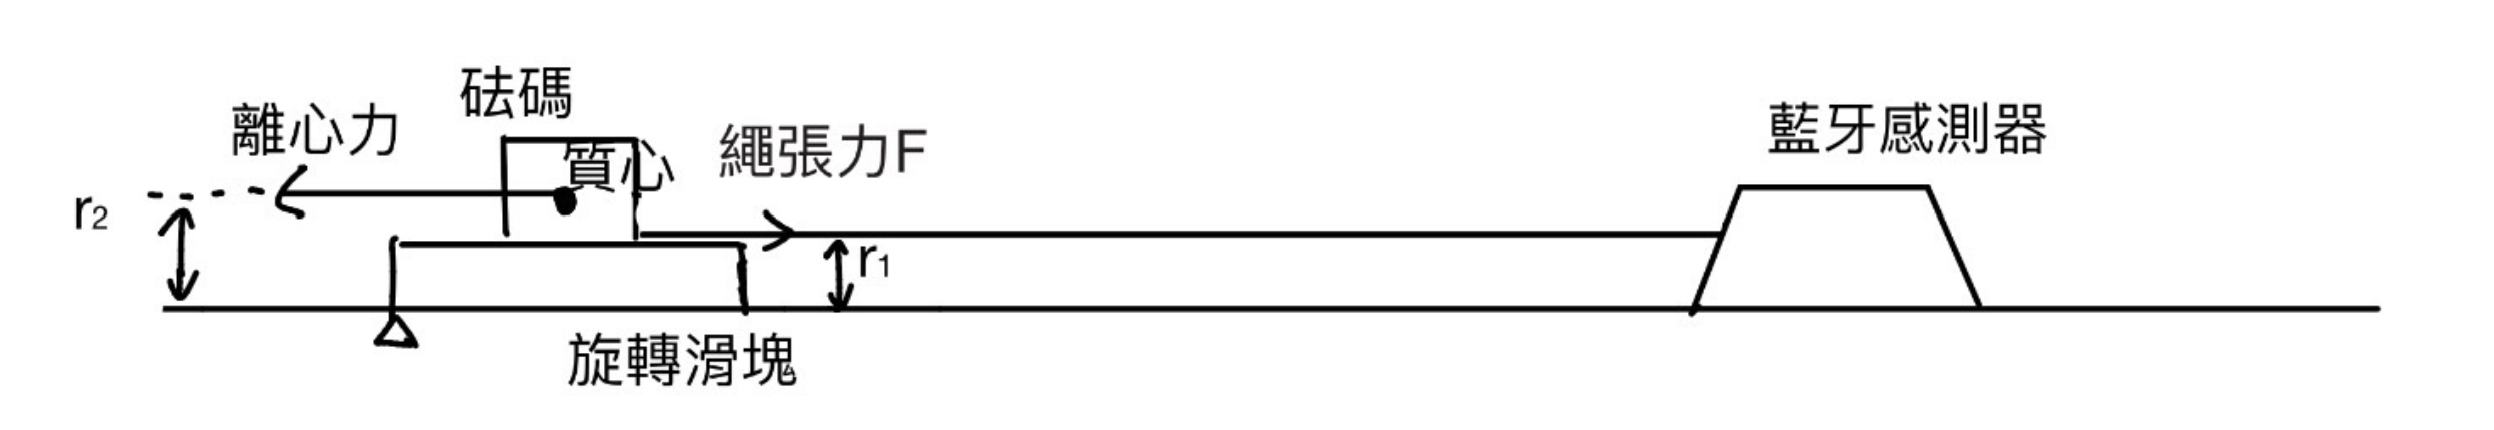
\includegraphics[width=0.8\textwidth]{翻轉假設示意圖.png}
                \caption{翻轉假設示意圖。此圖以旋轉滑塊為觀察者,考慮其離心力作用在質心,與鐵架垂直高度為$r_2$ 其中 $F$ 為纜線繩張力,與鐵架垂直高度為$r_1$。考慮加上砝碼的旋轉滑塊的真實形狀,推測$r_1 > r_2$。故繩張力必須要大於離心力$mr\omega^2$才不會讓砝碼和旋轉滑塊以左下角為支點做逆時針旋轉。}
                \label{fig:翻轉假設示意圖}
            \end{figure}            
            
            參考 \autoref{fig:翻轉假設示意圖},不考慮纜繩傾斜,以旋轉滑塊左下角為支點力矩平衡的方程式為

            \begin{gather}
                F r_1 = mr\omega^2 r_2
            \end{gather}

            因為摩擦力通過支點,不必計算。同時考慮角度和力矩稍微複雜。因為我們在實驗時皆有確認過纜繩無垂直方向的傾斜,而無法改變水平方向的傾斜。故我們以纜繩僅有水平方向傾斜,以及推測$1.05 r_1 = r_2$作為分析假設。

            \begin{gather}
                F r_1 \cos{\theta} = mr\omega^2 r_2\\
                \Rightarrow F = 1.05 \times \frac{mr\omega^2}{\cos{\theta}}
            \end{gather}

            根據此方式計算出的 $\theta$ 在實驗A為

            \begin{equation}
               \theta = \arccos\left( \frac{1.05}{1 + 0.056} \right) = \ang{6.111}
            \end{equation}

            而在實驗B則為

            \begin{equation}
               \theta = \arccos\left( \frac{1.05}{1 + 0.13} \right) = \ang{21.7}
            \end{equation}

            經過後,傾斜角讀較符合常理。考慮兩者的質心位置、傾斜角度可能不同,這只是一個定性的假設,然而經過簡單的假設和計算我們了解到這三個斜率的正偏差可以用這兩個假設(纜繩傾斜假設、翻轉假設)來解釋。

            而對於實驗C,\autoref{fig:實驗C數據 Excel原始數據}的斜率和不考慮摩擦力的情況吻合,即斜率與不考慮摩擦力的理論斜率 $r\omega^2$僅相差 0.8\% 因此我們推測本實驗更適用於本節提到考率的$F r_1 \cos{\theta} = mr\omega^2 r_2$,而$r_1/r_2$及${\cos{\theta}}$都相當接近一,即系統誤差很小。

        \subsection{實驗A、實驗B截距之討論}

            正如上一節所述,若我們考慮力矩平衡,則摩擦力實際上取決於角速度、$r_1/r_2$且不會列入計算的方程式,由第一節提到假設平衡時的摩擦力為最大靜摩擦力的假設,我們實驗A會算出負的摩擦係數,而實驗B算出的摩擦係數則為0.94,明顯大於兩個金屬之間的正常摩擦力。再者,我們為了避免儀器誤差,選用較大的角速度、旋轉半徑進行實驗,因此實驗數據分布並沒有接近原點,故截距之計算會有較大的誤差。綜上述原因,我們認為以這三個實驗無法求出摩擦係數。

        \subsection{實驗C截距之討論}

            \par
            本實驗不論以力矩$F r_1 \cos{\theta} = mr\omega^2 r_2$或力平衡的$F = m(r\omega^2 - g \mu)$,其力對質量作圖的理論截距皆為0。我們推測可能是有某地方有「卡住」或「黏住」正向力無關的摩擦力$f_0$,使得$F = m(r\omega^2 - g \mu) - f_0$,由 \autoref{fig:實驗C數據 Excel原始數據} 的截距得 $f_0 = \SI{0.33}{\newton}$。
        
    \section{結論}


    \printbibliography

\end{document}
